\documentclass[12pt]{article}
\usepackage[utf8]{inputenc}
\usepackage[letterpaper]{geometry}
\usepackage{times}
\usepackage{graphicx}
\usepackage{setspace}

\geometry{top=1.0in, bottom=1.0in, left=1.0in, right=1.0in}

\doublespacing

\begin{document}

    \begin{titlepage}
    \begin{center}
        \vspace*{4cm}

        \Huge
        \textbf{ECE-388}
        
        \Large
        \vspace{0.5cm}
        Lab 3: Pattern Generator 
        
        \vspace{8.5cm}
        \textbf{Marcel Vieira}
    
        November 22, 2020
        
        \small
        \vspace{0.5cm}
        I Marcel Vieira certify that this is lab report consists only of work that is my own.
        
    \end{center}
\end{titlepage}
    \tableofcontents
    \listoffigures
    \newpage

    \section{Abstract}

    This document describes the process taken in planning designing and constructing a pattern generator. The steps detailed currently include identification and defining the problem, creating a bill of materials, creating simulations, prototyping, and drafting PCB design layouts. This document also details the problems encountered along with how they were solved or proposed solutions. Due to the project still being worked on this document serves to document the progress.

    \section{Problem Statement}

    Use surface mount components and a ATMEGA 328pb to generate binary patterns at either 5V or 3.3V, with a user interface that allows a user to change the pattern as well as the logic level across 8 channels. 

    \section{Procedures}
        \subsection{Materials}

            \begin{itemize}
                \item Multisim
                \item Eagle
                \item Web Browser
                \item Atmel Studio
            \end{itemize}

        \subsection{Test Process}
        In order to begin the process of creating a pattern generator the problem must be properly defined to set the guidelines for what the solution will be. To define the problem the constraints must be laid out in an Engineering note book and clarified with the TAs and professor. They required that the ATMEGA328PB chip be used, and all components that are chosen must be surface mount. These two constraints are not enough to clearly define the problem so more must be added such as an ability to switch logic levels and a user interface that allows people to interact with the board and adjust the the output pattern. Now the problem can be defined with a problem statement, in this case it is done with the one above.
        \par Begin brain storming possible ways to resolve the problem. The ATMEGA328PB is capable of outputting digital signals in patterns so one of the biggest issues is changing the 5V is outputs from 5V to 3.3V when desired. This could be done with a dc converter, using resistors or diodes to drop the voltage, or using MOSFETS to toggle the flow of electricity form whatever logic source is selected. The second issue is in getting the 3.3V form the 5V that will come into the board. This could be done using a voltage divider, a DC to DC converter, or a Zener diode. The third issue was how was the user interface going to be made. The interface could be made either using hard ware switches, buttons, and rotary encoders or use serial port to type in the pattern. The last problem was how was information going to be shown to the user? The information could be shown using as series of LEDs or on a screen.
        \par The next step is to decide which brainstormed solutions will be used to solve the problem. For this project the user interface will use a serial input with a screen for the display. For the power logic level selection a Zener diode will be used to get the 3.3V with a sp3t switch to switch between the power states which will include 5V 3.3V and 0V. The voltage that comes out of the switch then will be passed to MOSFETS that will be toggled by the ATMEGA328PB chip.
        \par Now that the plan has been completed the parts must be selected and tested in Multisim (figure 1). For this case the displays cannot be properly tested so they will be tested physically later on. The MOSFETS when input in Multisim showed that the were capable of using 5V at the gate to toggle both 5V and 3.3V. The Zener diode also showed it was a valid solution to getting 3.3V.

        \begin{figure}[htp]
            \centering
            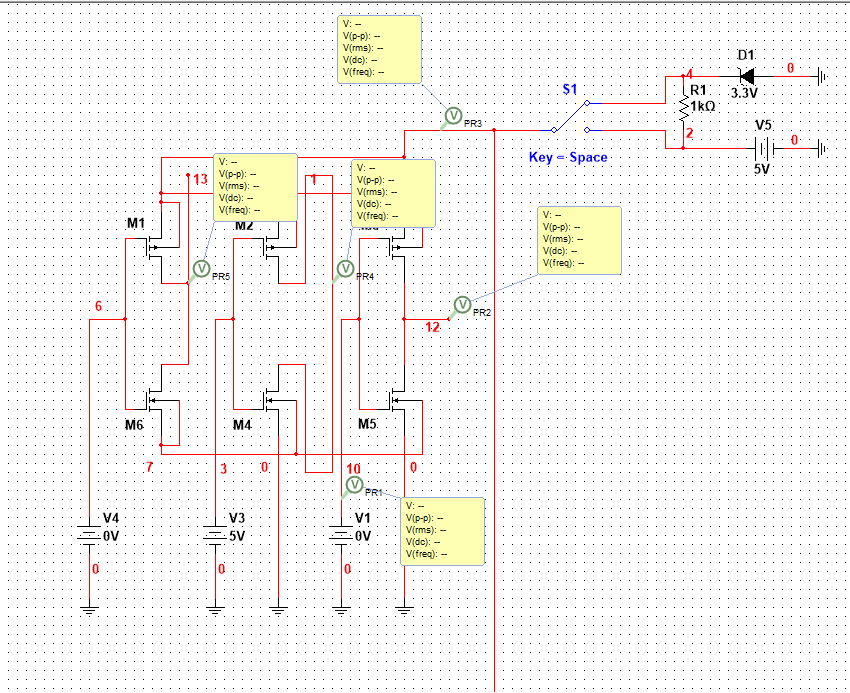
\includegraphics[width=8cm]{Pattern Gen Multisim V1.png}
            \caption{Pattern Gen Multisim V1}
        \end{figure}

        \newpage

        \par Then the parts that are required to build the circuit are searched in LCSC and Digikey. When a part was found it was inserted into Eagle (figure 2). Once all the parts were placed in Eagle a bill of materials is exported and opened in excel in order to add purchase information and remove irrelevant information (figure 3).

        \begin{figure}[htp]
            \centering
            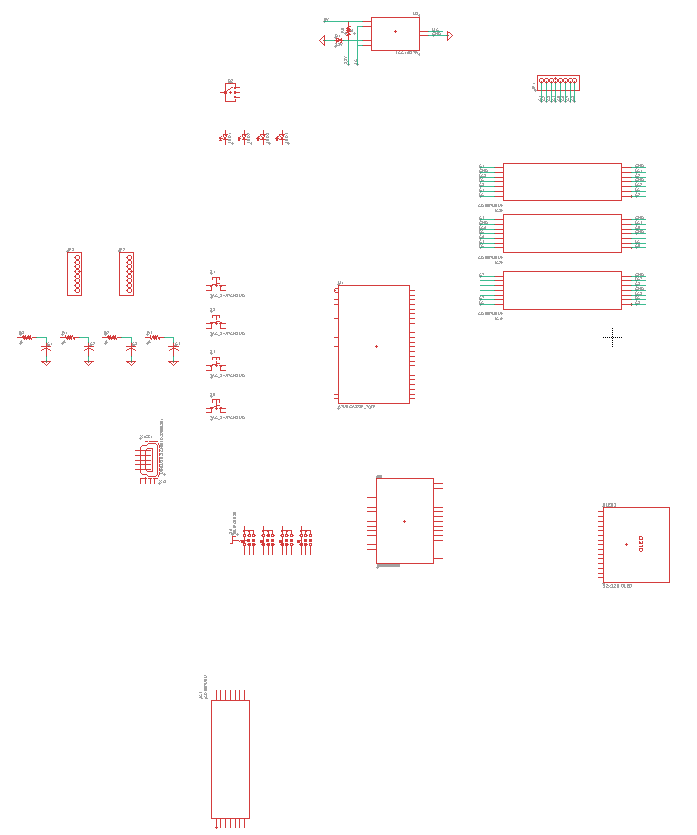
\includegraphics[width=8cm]{Pattern Gen Eagle V1.png.png}
            \caption{Pattern Gen Eagle Schematic V1}
        \end{figure}

        \begin{figure}[htp]
            \centering
            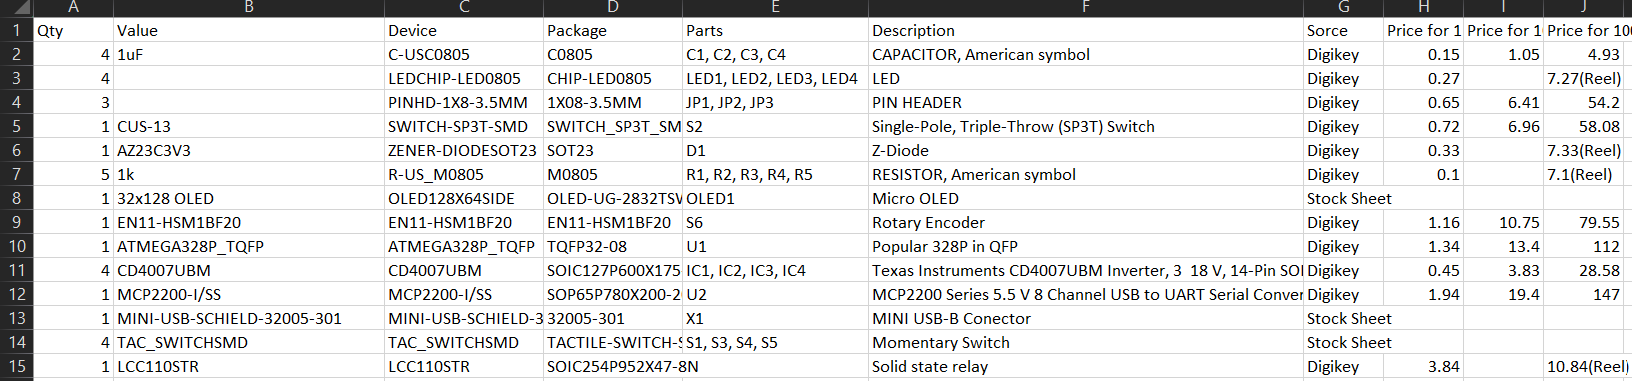
\includegraphics[width=8cm]{BOM1.png}
            \caption{Pattern Gem BOM 1}
        \end{figure}

        \newpage

        \par After the parts were selected and the circuit was successfully simulated it was time to begin construction of the prototype. The prototype allows for the circuit to be tested prior to having everything on the PCB. The use of a prototype especially one on a bread board allows for parts to be more easily isolated and replaced.The the prototype is constructed based on the circuit design used in Multisim but the prototype is broken into sections to test the functionality of all the individual smaller parts prior to testing the circuit in its entirety. The prototype consisted of a voltage regulator, a switching circuits made with 2 PMOSs and an inverter, and a set of CMOS inverters.
        \par The first test conducted was connect a voltmeter to the the voltage regulator and check if the proper voltages are produced. The expected values were 5V at the input and 3.3V at the output. This ensures that the voltage does not damage the circuit and sets a base line for the voltage to expect in the inverters. 
        \par The second test is to put 5V and 3.3V to the switching circuit use the voltmeter to check if it is outputting the correct input depending on what signal is sent to it. If a high is put into the circuit it should output 3.3V, if a low is put into the circuit it should output 5V.
        \par The final test for the first prototype was to check if the CMOS inverters could produce the expected signal. To test this a clock pulse is put into the inverter and the response as well as the input are measured and compared with an oscilloscope. The result showed be the opposite of the input with the exception of the high being what voltage is put to the sources of the PMOSs in the CMOS inverters.
        \par After taking notes on the first prototype the second was built. This prototype is focused on the user interface. This prototype consists of a rotary encoder with a built in button, several LEDs, and a 328pb. For this prototype code was written in Atmel Studio. The code for the prototype used various interrupts with 2 pin change interrupts being used to determine the direction the rotary encoder is turned on. There is also another pin change interrupts that is used to change the button press. This user interface was tested using debugging and visual observation to tell whether it is operational. 

        \begin{figure}[htp]
            \centering
            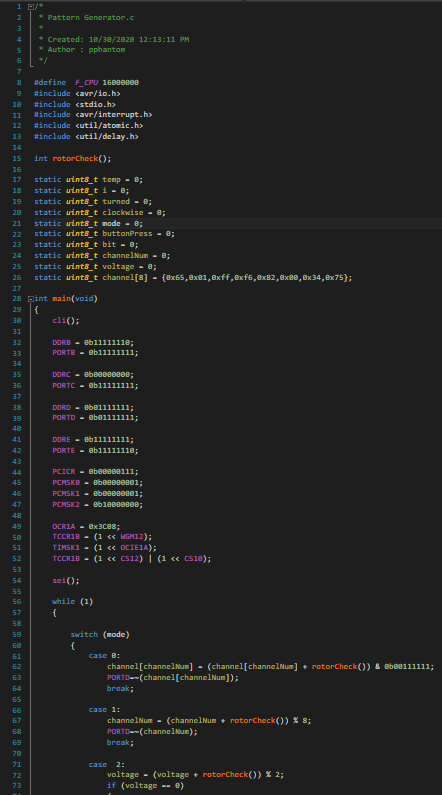
\includegraphics[width=8cm]{Pattern Gen Code V1 PG 1.png}
            \caption{Pattern Gen Code V1 PG 1}
        \end{figure}

        \begin{figure}[htp]
            \centering
            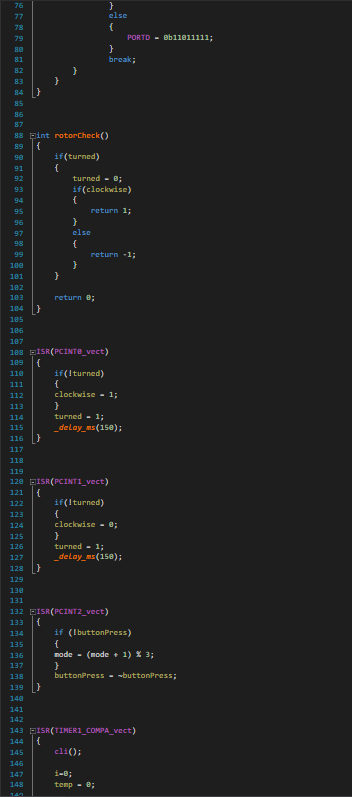
\includegraphics[width=8cm]{Pattern Gen Code V1 PG 2.png}
            \caption{Pattern Gen Code V1 PG 2}
        \end{figure}

        \par The user interface should have LEDs that start off displaying the current binary signal, this is referred to as mode 1. In mode 1 the rotary encoder changes the binary value going up when turned clockwise and down when turned counter clockwise. When the button is pressed it enters mode 2 which allows the user to view the the current channel number in binary displayed on the LEDs. Mode 2 also allows for the user to switch between channels using the rotary switch. When the button is pressed again it goes into mode 3 which simulates the display of the voltage settings which is adjustable with the rotary encoder as well.
        \par Once the final design has been decided on the the design must properly be translated into a schematic that will be uploaded to Github and checked by Tim Chase. The schematic must contain all parts that are to be used, in this instance that would be the micro USB, the CMOS chips, the serial chip, the LEDs, the OLED display, and the rotary encoder. Power must flow in the schematic from the left to right and be clearly labeled. The schematic must finally pass all ERC checks with no errors or only errors approved by Tim Chase. 
        \par Once the schematic is approved by Tim Chace the board lay out can then be worked on. The board layout must include all parts, ground planes, fiducials to show the alignment of the board, and must pass all DRC checks in the file Dirty8TS.dru. On the back of the board the board must have a name, date, version number, and the Git repository link printed on the back of the board.


    \section{Discussion}
    Originally the circuit was going to use a voltage divider to drop the voltage to 3.3V, and N-type MOSFETS to toggle to logic voltages on and off but they presented several issues in the Multisim simulations. For the voltage divider applying the 3.3V to a load changed the resistance on altering the voltage and because the resistance was going to be difficult to predict the Zener diode was used. For the N-type MOSFETS they worked perfectly but each of the MOSFETS was there own chip, but after a suggestion by Tim Chace CMOS inverters were used instead which proved to be just as affective and required 3 times less chips saving space. These test processes lead to the revision of the bill of materials 3 times.
    \par For prototyping all test ran as expected proving that all systems individually are operational. This is with the exception of the linear regulator, the MCP2200 serial chip, and the OLED display.
    For the display and serial chip they have not come in time to be properly tested, but the voltage regulator was tested and failed. The failure at first was due to the wrong chip being supplied without a part number which meant that the wrong data sheet was used to wire the chip. This in turn damaged the chip and because there was only one further tests could not be done. An attempt was made to test a complete prototyping but there were complications with the 328pb which made it unable to be identified by any computer. This resulted in the 328pb not being able to be programmed. This caused the loss of another test session. Fortunately Ben Vial was able to repair the board so even if the issue occurs again there is a know solution for the problem now.
    \par In creating the first schematic a new USB and an OLED were added to the schematic that originally only contained parts. After wiring the schematic several issues presented themselves. First the resonator that was attached to the previous schematic was the wrong size. The second issue was that there were no power labels connected. Once these corrections were made even more issues appeared. These issues were brought up by Ben Vial that let students know that the OLED display runs on 3Vs while the 328pb runs on 5V in order. To eliminate issues with communication between the 2 chips he recommended incorporate a MOSFET level shifter. After fixing this the USB had to be replaced with one that had a similar foot print to what was  in the stock sheet.
    \par Once the schematic was all set all focus was paced on completing the layout. The issues that were worked on for the layout focused more on labeling and having correct foot prints for all components. Fiducials were also added to the layout to indicate proper orientation. While replacing one of the components in the layout it disappeared but still appeared in the schematics the rest of the time working on the boards were centralized around attempting to resolve the issues. After the third attempt the entirety of the board was populated by the correct parts.  
    

    \section{Conclusion}
    For the bill of materials it is completed but it still may change because no solution has been found to electronically switch between the sources being used for the logic levels. There are still issues with the voltage regulator and a full prototype replicating the entire system must still be tested. The schematics and board layout have been completed but are still awaiting approval before it can be sent to the manufacturer.

    \section{Reflection}
    The planning and simulation had no major issues. There only three minor issues. The first was that it was unclear early on what the pattern generator was and what it was supposed to do.The second was that simulating the circuits proved difficult at first because the necessary chips were not in Multisim so they had to be built out of equivalents that had to be found in Multisim. The third issue was that no clear way to use the MOSFETS to switch between logic sources was found.
    \par In the prototyping stage one of the major issues was a lack of parts to work with which caused a lot of time to be lost and a lot of confusion. This problem was difficult to avoid due to the current pandemic and the restrictions placed as a consequence. Another issue encountered with prototyping was time management. Due to issues with the regulator a majority of lab time was spent around trouble shooting it. Because so much time was lost the rest of the test were done quickly and pictures were not taken. This is why there are no images of the first and second prototyping stages.
    \par The process of creating a final schematic and board lay out came with unexpected issues. One of the major issues was communication. Due to the time constraints being so tight it was difficult to make changes and get the revised quickly. The biggest issue was due to a lack of understanding of what was on the write up that detailed the requirements of the schematic and layout. To solve this issue other students were consulted and they were able to clarify what was needed. In the future other students will be contacted sooner in the event of confusion.

\section{Appendix}

\begin{figure}[htp]
    \centering
    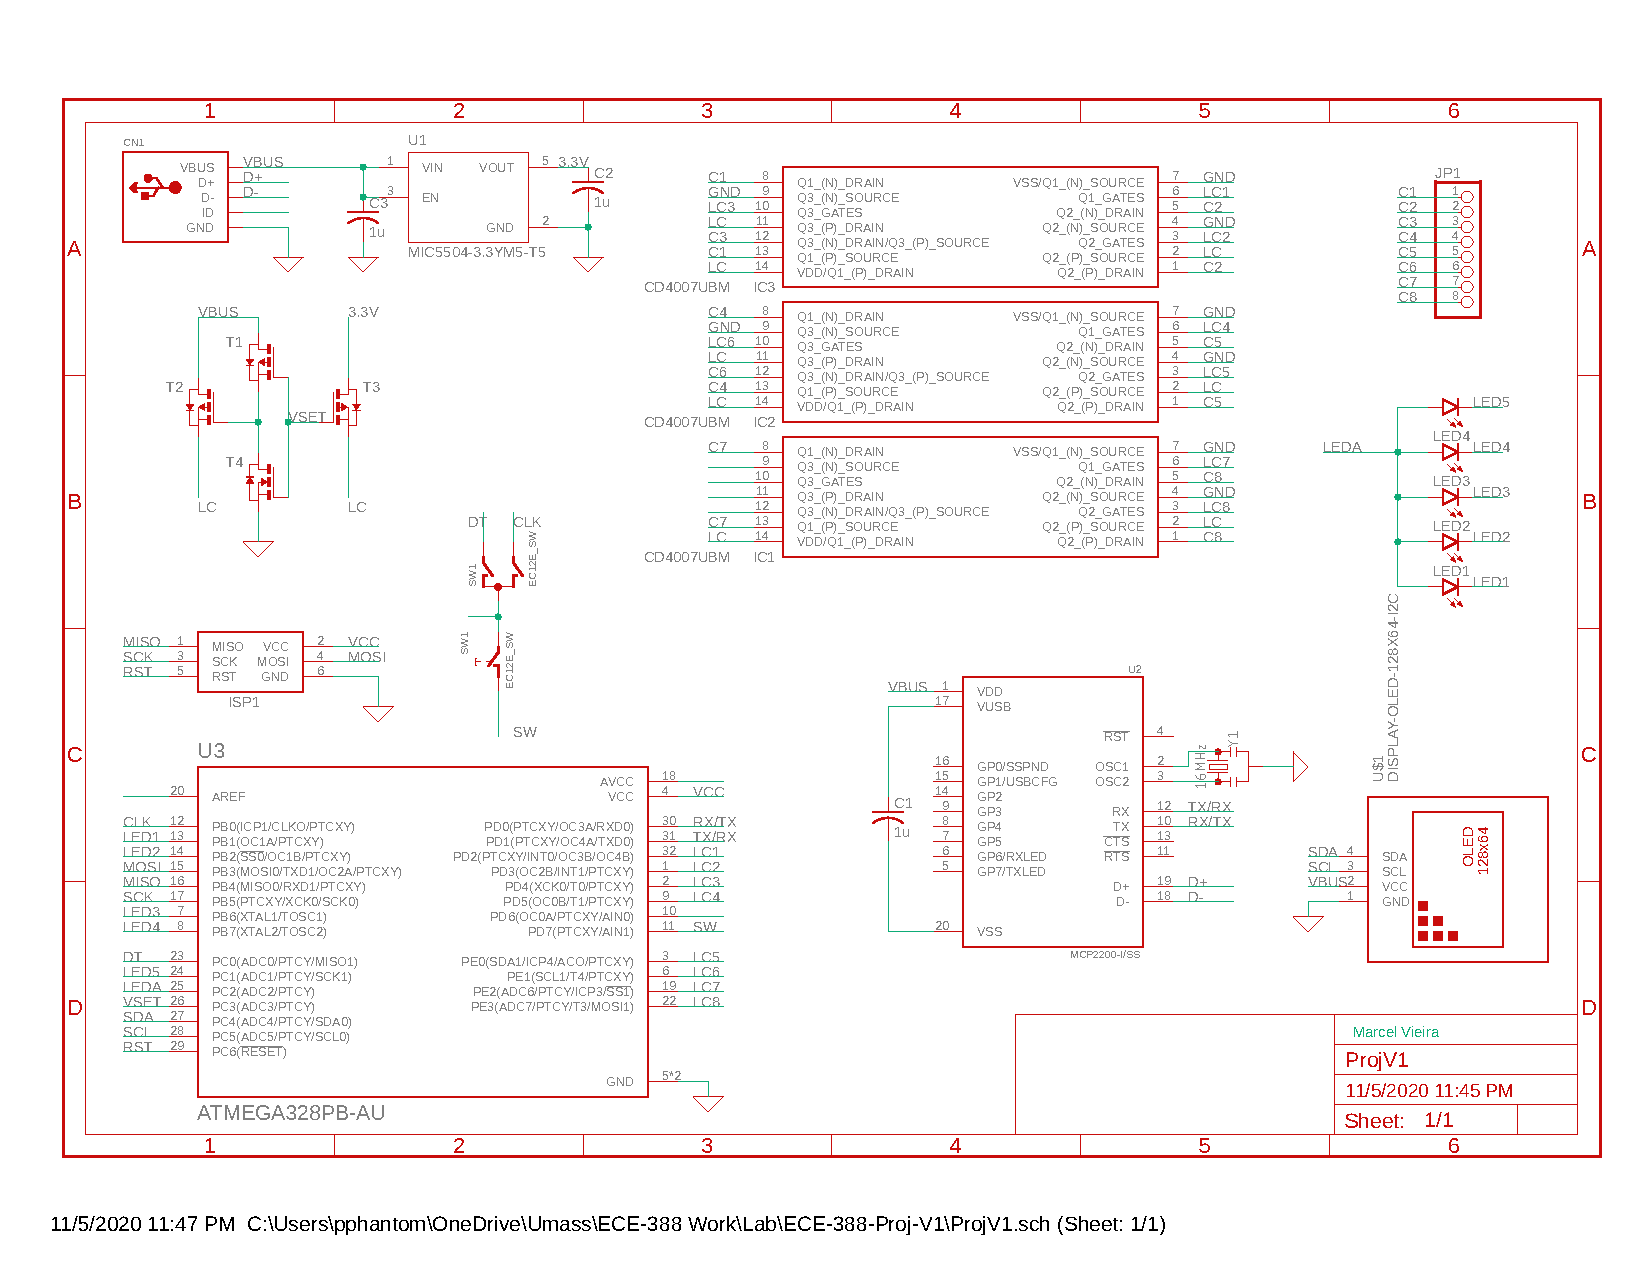
\includegraphics[width=10cm]{ProjV1.pdf}
    \caption{Schematic V1}
\end{figure}

\begin{figure}[htp]
    \centering
    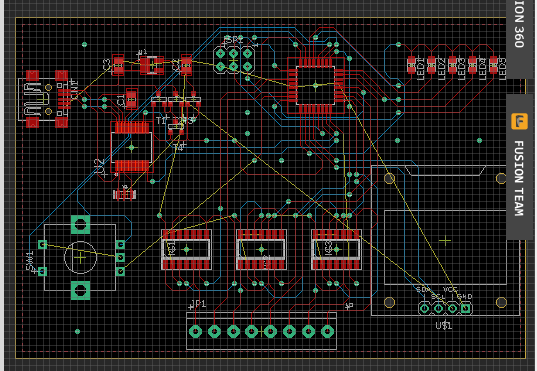
\includegraphics[width=10cm]{LayoutV1.png}
    \caption{Layout V1}
\end{figure}

\begin{figure}[htp]
    \centering
    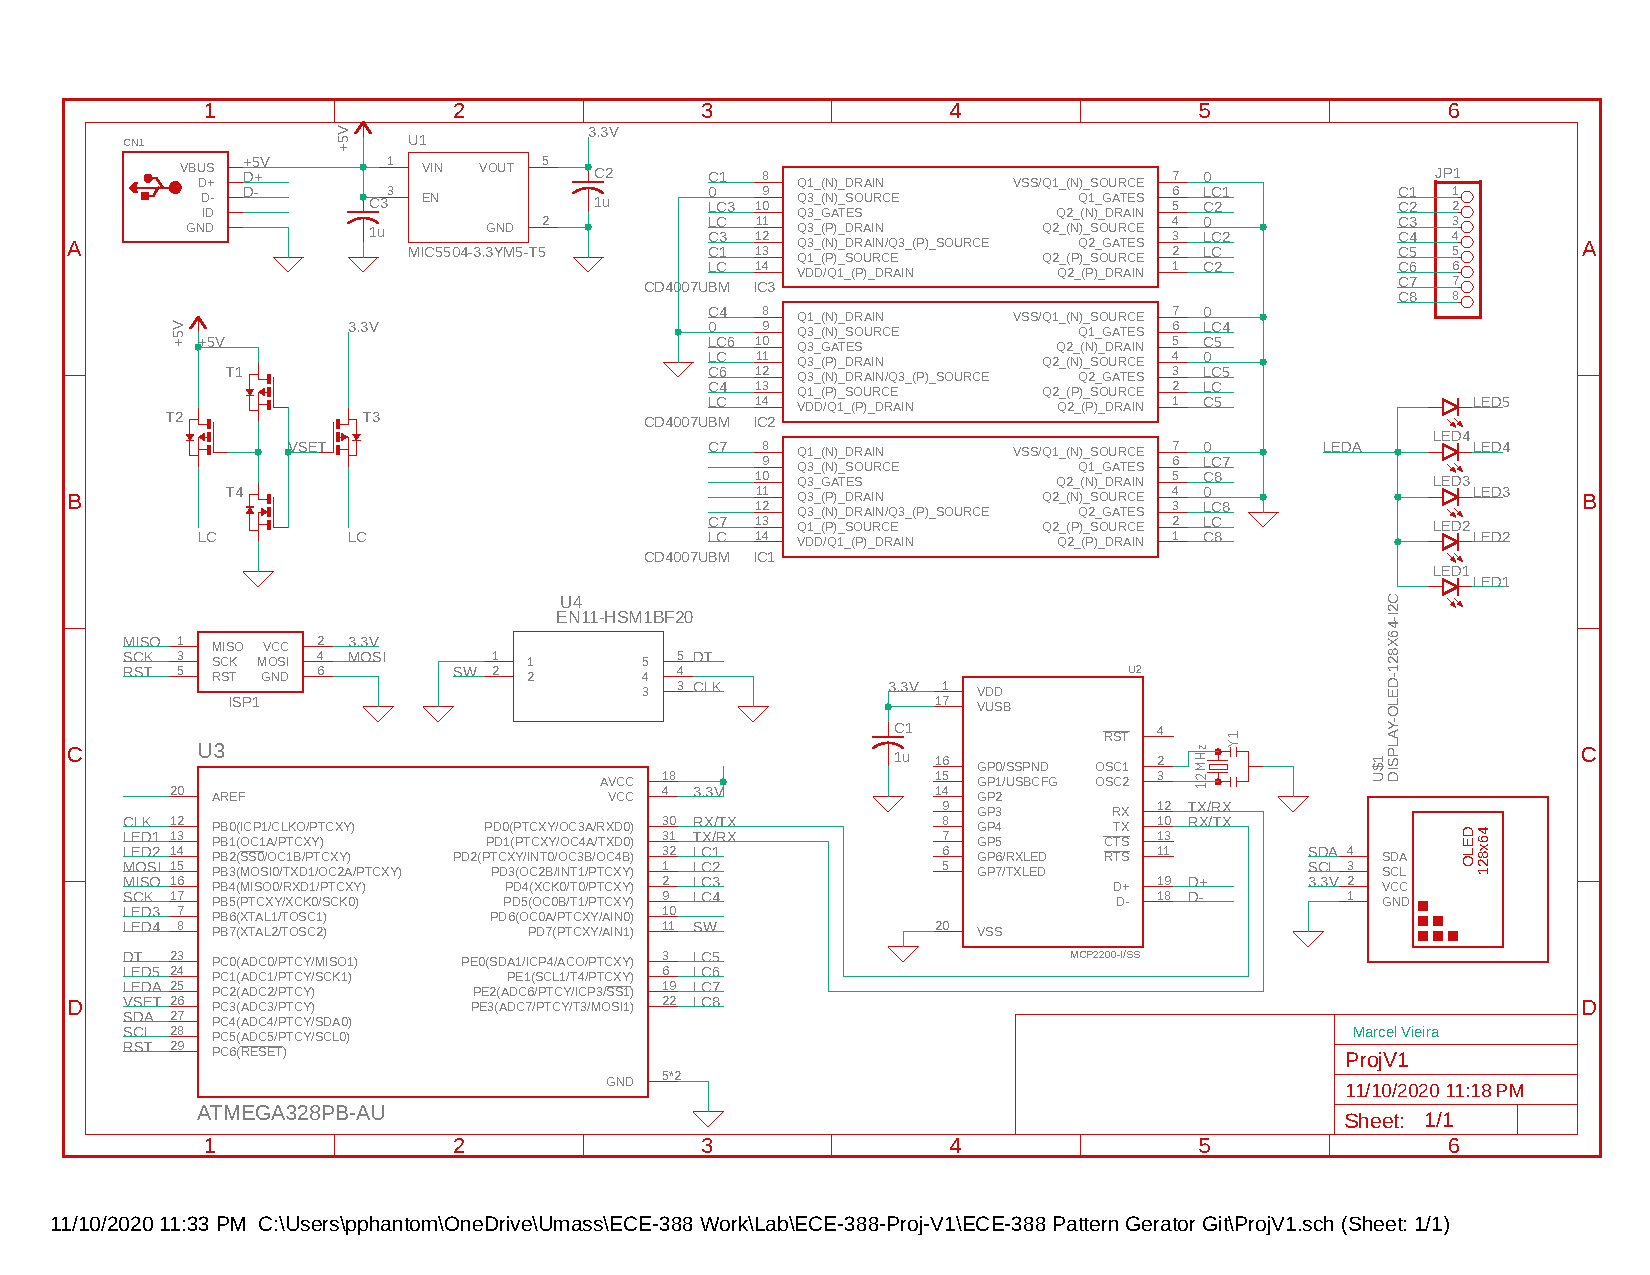
\includegraphics[width=10cm]{ProjV2.pdf}
    \caption{Schematic V2}
\end{figure}

\begin{figure}[htp]
    \centering
    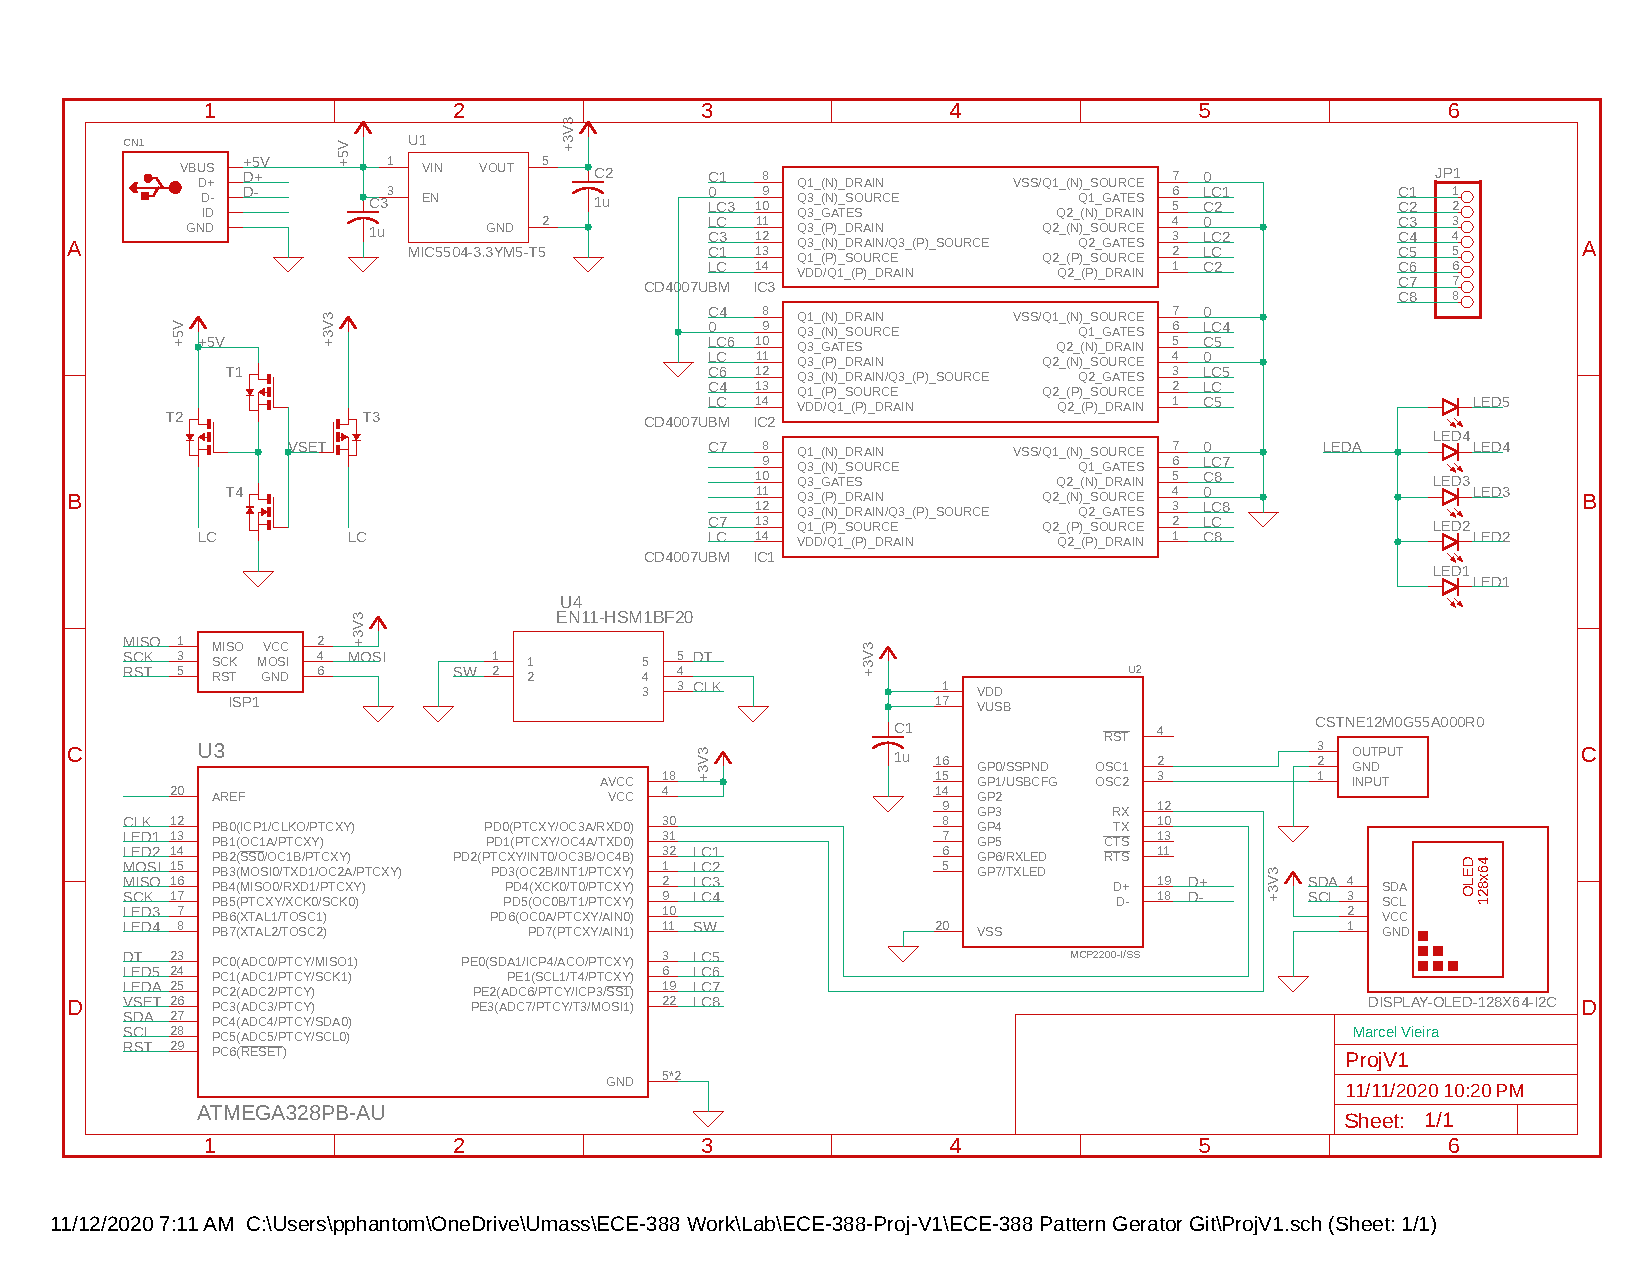
\includegraphics[width=10cm]{ProjV3.pdf}
    \caption{Schematic V3}
\end{figure}

\begin{figure}[htp]
    \centering
    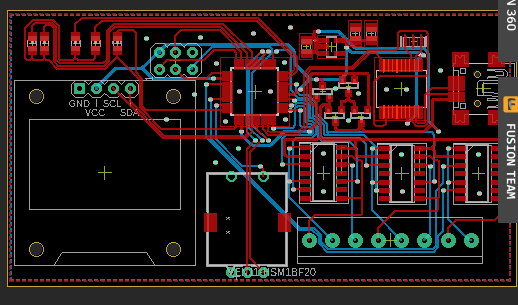
\includegraphics[width=10cm]{LayoutV3.png}
    \caption{Layout V3}
\end{figure}

\begin{figure}[htp]
    \centering
    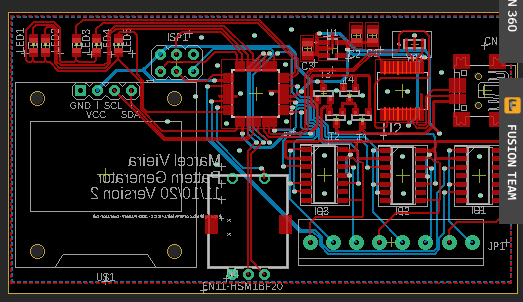
\includegraphics[width=10cm]{LayoutV4.png}
    \caption{Layout V4}
\end{figure}

\begin{figure}[htp]
    \centering
    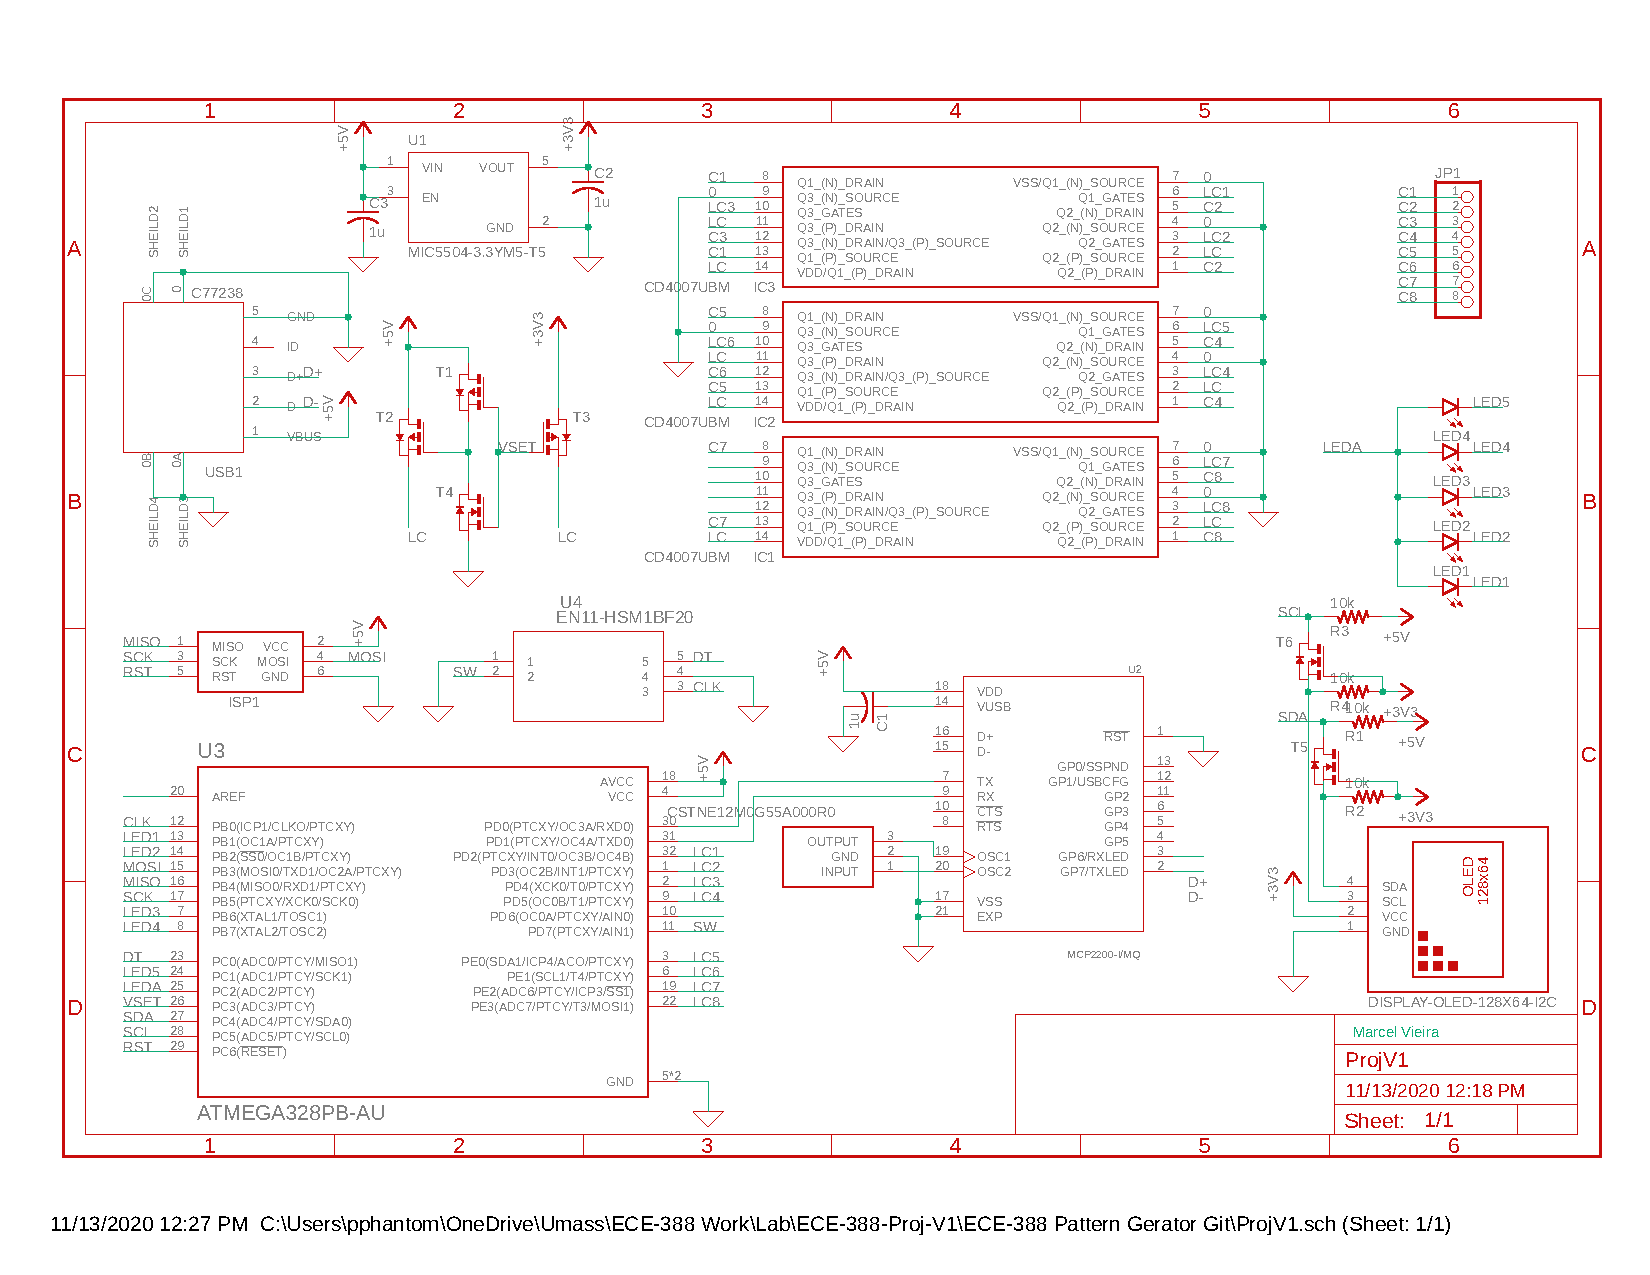
\includegraphics[width=10cm]{ProjV5.pdf}
    \caption{Schematic V5}
\end{figure}

\begin{figure}[htp]
    \centering
    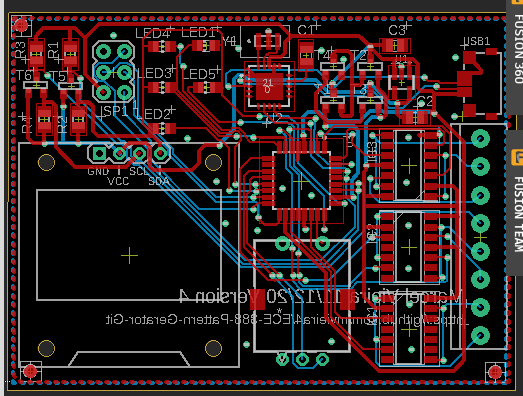
\includegraphics[width=10cm]{LayoutV5.png}
    \caption{Layout V5}
\end{figure}

\end{document}
